\begin{figure}[H]
    \centering

\begin{tikzpicture}
\pgfplotsset{
    every axis/.style={ymin=0},
    width=0.22\textwidth,
    height=0.25\textheight,
    xtick={2, 3, 4, 5, 6, 7, 8, 9, 10},
    y axis style/.style={
    yticklabel style=#1,
    ylabel style=#1,
    y axis line style=#1,
    ytick style=#1}}
\begin{axis}[ scale only axis, ymin=500, xmin=2,xmax=10, axis y line*=left, xlabel=Number of Cores, ylabel=Execution time (s), y axis style=green!75!black]
    \addplot[smooth, green!75!black, mark=o, draw] 
    coordinates 
    {
        (2,748)
        (3,698)
        (4,676)
        (5,667)
        (6,655)
        (7,660)
        (8,656)
        (9,654)
        (10,654)
    };
\end{axis}
%
\begin{axis}[ scale only axis, ymin=4000, xmin=2,xmax=10, axis y line*=right, axis x line=none, ylabel=DEC (j), y axis style=blue]%
    \addplot[smooth, blue, mark=x] 
    coordinates 
    {
        (2,6619)
        (3,6392)
        (4,6305)
        (5,6265)
        (6,6221)
        (7,6235)
        (8,6207)
        (9,6184)
        (10,6184)
    };
\end{axis}
%
\begin{axis}[red, scale only axis, ymin=3, ymax=5, xmin=2,xmax=10, axis y line*=right, axis x line=none, ylabel=DEC per second (w)]%
\pgfplotsset{every outer y axis line/.style={xshift=2cm}, every tick/.style={xshift=2cm}, every y tick label/.style={xshift=2cm} }
    \addplot[smooth, red ,mark=+] 
    coordinates 
    {
        (2,3.7569774032360472)
        (3,4.105360236705367)
        (4,4.2727454208041555)
        (5,4.3467751739782)
        (6,4.449545186403633)
        (7,4.383316849780688)
        (8,4.428382630501816)
        (9,4.404787243303039)
        (10,4.413873085504976)
    };
\end{axis} 

\end{tikzpicture}
    \caption{The evolution of the DEC (blue), DEC per second (red) and execution time (green) as more cores are allocated to PCM on DUT 2. Note that the x- and y- axis does not start at zero.}
    \label{fig:exp_3_dut_2_pcm_result}
\end{figure}